\cleartooddpage[\thispagestyle{empty}]
\chapter{Vortex Analysis to predict IA Initiation}\label{CHAPTER3}

The tangential, frictional stress caused by blood flowing along the vessel wall is known as WSS. The ANSYS-FLUENT software calculates WSS by the normal velocity gradient at the vessel wall:
	\begin{equation}
\tau\textsubscript{w} = \mu\frac{\partial v}{\partial n}
	\end{equation}
where $\mu$ is the dynamic viscosity. In this work, areas of high WSS were of interest as it is thought to play a role in the IA initiation \cite{Meng1254}. High WSS was defined as values $\ge$ 20 Pa during peak systole of the MRI waveform.

The WSSG was calculated using in-house VMTK scripts and is derived from three spatial derivatives of the WSS as follows:
	\begin{equation}
WSSG = \sqrt{(\frac{\partial{\tau_{w}}}{\partial{x}})^2 + (\frac{\partial{\tau_{w}}}{\partial{y}})^2 + (\frac{\partial{\tau_{w}}}{\partial{z}})^2}
	\end{equation}
with the time-averaged WSSG calculated as
	\begin{equation}
WSSG\textsubscript{av} = \frac{1}{T}\int_{0}^{T} | WSSG | dt
	\end{equation}
	
OSI is a nondimentional parameter, computing oscillations in the direction of the WSS vectors over the course of a cardiac cycle:
	\begin{equation}
OSI=\frac{1}{2}\left\{1-\frac{| \int_{0}^{T} \mathrm{\tau}_{i}dt |}{\int_{0}^{T} | \mathrm{\tau}_{i} | dt}\right\}
	\end{equation}
were $\tau\textsubscript{i}$ represents the WSS vector at a given time step across the duration of the cardiac cycle (T). The OSI describes the changes of a WSS vector's alignment with the cardiac cycle's temporally-averaged WSS vector. An OSI of 0 indicates no change in directionality and 0.5 being a complete direction reversal. 

The AFI \cite{Mantha1113} quantifies the variation in angle between the instantaneous WSS vector and time-averaged WSS vector:
	\begin{equation}
AFI=cos(\theta)=\frac{\mathrm{\tau}_{i}\cdot \mathrm{\tau}_{av}}{| \mathrm{\tau}_{i} |*| \mathrm{\tau}_{av}|}
	\end{equation}
For each point along the vessel wall, the minimum AFI calculated during the cardiac cycle was used to indicate the greatest deviation of the WSS vector from its mean direction. A minimum AFI of -1, 0, and 1 indicate deviations of 180\textdegree, 90\textdegree, and 0\textdegree respectively.

The GON index \cite{Shimogonya2009} quantifies fluctuations in WSSG directionality over the cardiac cycle. 
	\begin{equation}
GON=1-\frac{|\int_{0}^{T}Gdt|}{\int_{0}^{T}| G | dt}
	\end{equation}
T is the period of the cardiac cycle and G is the spatial wall shear stress gradient vector



Lorem ipsum dolor sit amet, at qui viderer recusabo aliquando, dignissim 
evertitur ei his. Ignota iuvaret fabulas ei vim. Ne utinam inciderint quo. 
Pri ea congue postulant conclusionemque. In prima quaeque diceret pri. Enim 
labores contentiones eos at, duo altera denique nominavi ea, eos inani 
nominavi consectetuer at. Ut elitr dicam elaboraret pro, ius altera 
voluptaria cu.

Discere dissentiet vel et, soluta nostrum epicurei ad eam, cu has aperiam 
vituperata. In prima quaeque diceret pri. Enim labores contentiones eos at, 
duo altera denique nominavi ea, eos inani nominavi consectetuer at. Ut elitr 
dicam elaboraret pro, ius altera voluptaria cu. Eam mazim aliquip cu, 
recusabo pericula accommodare at mea, facer affert nonumes qui ea.
\cite{LAPACK_00,FFTW3_00}

\begin{align*}
  d\nu_\theta &\;=\; \frac{N}{V}\:\left( \frac{m}{2\pi\:kT} \right)^{3/2}\;
                    \left[\int_{0}^{2\pi}\:\int_{0}^{\infty}\:v^3\:e^{-mv^2/2kT}\:dv\:d\phi \right]\;
                    \sin\theta\;\cos\theta\;d\theta \\\\
              &\;=\; 2\:\pi\;
                    \frac{N}{V}\:\left( \frac{m}{2\pi\:kT} \right)^{3/2}\;
                    \left[\int_{0}^{\infty}\:v^3\:e^{-mv^2/2kT}\:dv\: \right]\;
                    \sin\theta\;\cos\theta\;d\theta
\end{align*}

At vix indoctum disputando. Eam cu doctus reprimique, quaeque democritum 
an eos, sit veniam facete dissentias id. Tale volumus eos te, an eum nulla 
tincidunt. Mea id recteque theophrastus.
\begin{equation}
  d\nu_\theta \;=\; \frac{N}{V}\;\left(\frac{2\:k\:T}{m\:\pi} \right)^{1/2}\;
                  \sin\theta\;\cos\theta\;d\theta
  \label{CHAPTER3_EQN01}
\end{equation}

Liber liberavisse nec at, movet albucius principes has at. Ea sed persius 
accusam, clita sententiae adversarium ne sed. Usu no graecis theophrastus 
delicatissimi, sint aliquam an eam. Mei elit mnesarchum dissentias te, in 
essent laboramus per. Affert mucius quidam mel ex, per dicam insolens ad.

Sed altera placerat an, id verterem abhorreant 
interesset mea. Eum at ceteros efficiantur. Eos id voluptaria efficiendi 
comprehensam. Continuing from Eqn. \eqref{CHAPTER3_EQN01}

\begin{align*}
  d\nu_v &\;=\; \frac{N}{V}\;\left(\frac{m}{2\pi\:kT} \right)^{3/2}\;
               \left[\int_{0}^{2\pi}\;\int_{0}^{\pi/2}\;\sin\theta\;\cos\theta\;d\theta\;d\phi \right]\;
               v^3\:e^{-mv^2/2kT}\;dv \\\\
         &\;=\; 2\;\pi\;\frac{N}{V}\;
               \left(\frac{m}{2\pi\:kT} \right)^{3/2}\;
               \left[\int_{0}^{\pi/2}\;\sin\theta\;\cos\theta\;d\theta \right]\;
               v^3\;e^{-mv^2/2kT}\;dv
\end{align*}

In mel modo dicam vocibus, eruditi consectetuer vim no, cu quaestio 
instructior eum. Justo nostrud fuisset ea mea, eam an libris repudiandae 
vituperatoribus. Est choro corrumpit definitionem at. Vel sint adhuc vocibus 
ea, illud epicuri eos no. Sea simul officiis ea, et qui veri invidunt 
appellantur. Vix et eros ancillae pertinax.
\begin{figure}[htb]
  \begin{center}
    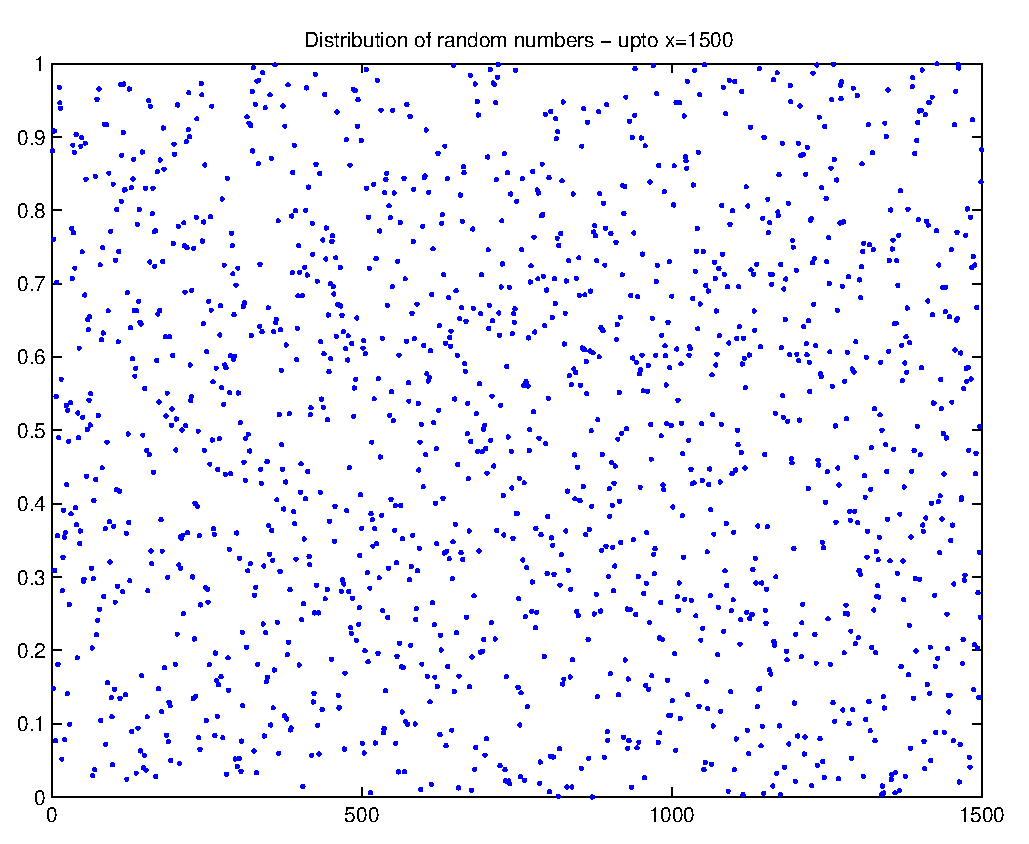
\includegraphics[width=0.95\textwidth]{RandomDistribution}
  \end{center}
  \caption{Distribution of random numbers}
  \label{CHAPTER3_FIG01}
\end{figure}

In mel modo dicam vocibus, eruditi consectetuer vim no, cu quaestio 
instructior eum. Justo nostrud fuisset ea mea, eam an libris repudiandae 
vituperatoribus. Est choro corrumpit definitionem at. Vel sint adhuc vocibus 
ea, illud epicuri eos no. Sea simul officiis ea, et qui veri invidunt 
appellantur. Vix et eros ancillae pertinax.
\begin{equation}
  d\nu_v \;=\; \frac{N}{V}\;\pi\;
               \left(\frac{m}{2\pi\:kT} \right)^{3/2}\;
               v^3\;e^{-mv^2/2kT}\;dv
  \label{CHAPTER3_EQN02}
\end{equation}

Aliquip lobortis ei est, at error viris graeco sed. Vel te elitr detracto, 
modo graecis scripserit ex nec. Errem utamur viderer per no, eam ea eripuit 
referrentur. Pro te dicat disputando.

\begin{table}[hbt]
  \caption{Measured data points representing the relationship between $x$ and
    $y$}
  \begin{center}
    \begin{tabular}{r|rrrrrrrrrrr}
      \hline
      $x$ & 0 & 1 & 2 & 3 & 4 & 5 & 6 & 7 & 8 & 9 & 10\\
      \hline
      $y$ & 0 & 0.94 & 0.99 & -0.52 & -1.82 & -0.44 & 3.54 & 6.69 & 5.38 & 0.00 & -4.42\\
      \hline
    \end{tabular}
  \end{center}
  \label{CHAPTER3_TABLE01}
\end{table}

Et mei mollis scripta, et vim labores phaedrum, in cum facete saperet. 
Splendide elaboraret comprehensam qui ne. Putant verterem no vim, mea solum 
veritus definitiones ei, no labitur propriae deseruisse est. Ius illud everti 
salutandi id, eu facer pericula principes est.

\begin{landscape}
  \begin{table}[hbt]
    \caption{A landscape table: 
      first column represents the year in which the Nobel prize in 
      physics was awarded; second column indicates the name of the 
      scientist and the third column is an \textsl{as is} Nobel
      citation}
    \begin{center}
      \begin{tabular}{p{0.40in}p{2.30in}p{4.85in}}
        \hline
        \multicolumn{1}{c}{\textbf{Year}} &
        \multicolumn{1}{c}{\textbf{Scientist(s)}} &
        \multicolumn{1}{c}{\textbf{Nobel Work}}\\
        \hline
        1901 & W. C. R\"{o}ntgen           & in recognition of the extraordinary services he has rendered by the discovery of the remarkable rays subsequently named after him\\
        1902 & H. A. Lorentz and P. Zeeman & in recognition of the extraordinary service they rendered by their researches into the influence of magnetism upon radiation phenomena\\
        1903 & A. H. Becquerel             & in recognition of the extraordinary services he has rendered by his discovery of spontaneous radioactivity\\
             & M. Curie and P. Curie       & in recognition of the extraordinary services they have rendered by their joint researches on the radiation phenomena discovered by Prof. Henri Becquerel\\
        1904 & J. W. Strutt                & for his investigations of the densities of the most important gases and for his discover argon in connection with these studies\\
        1905 & P. E. A. von Lenard         & Cathode rays\\
        1906 & J. J. Thomson               & Electrical conductivity of gases\\
        1907 & A. A. Michelson             & Spectroscopic and metrological investigations\\
        1908 & G. Lippmann                 & Photographic reproduction of colours\\
        1909 & K. F. Braun and G. Marconi  & Wireless telegraphy\\
        1910 & J. D. van der Waals         & Equation of state of gases and liquids\\
        1911 & W. Wien                     & Laws governing heat radiation\\
        1912 & N. G. Dal\`{e}n             & Automatic regulators for lighting coastal beacons and light buoys\\
        \hline
      \end{tabular}
      \label{CHAPTER3_TABLE02}
    \end{center}
  \end{table}
\end{landscape}

Et mei mollis scripta, et vim labores phaedrum, in cum facete saperet. 
Splendide elaboraret comprehensam qui ne. Putant verterem no vim, mea solum 
veritus definitiones ei, no labitur propriae deseruisse est. Ius illud everti 
salutandi id, eu facer pericula principes est.

\begin{figure}[htb]
  \begin{center}
    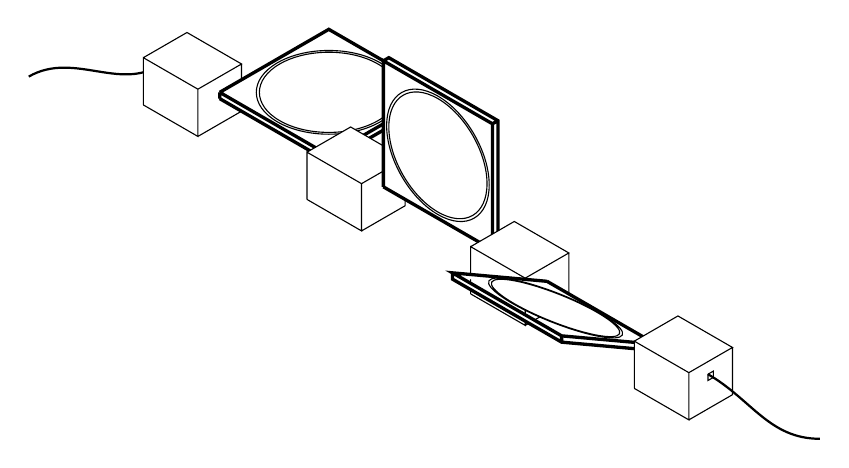
\begin{tikzpicture}[x={(0.866cm,-0.5cm)},
      y={(0.866cm,0.5cm)}, z={(0cm,1cm)}, scale=0.80]
      \tikzstyle{paddle}=[very thick, fill=white]
      \coordinate (O) at (0, 0, 0);

      % fiber in
      \draw[thick] (0,-1.5,0) to[out=30,in=220] (1,0,0);

      % first divider
      \draw[fill=white] (1,-.4,-.5) -- (2,-.4,-.5) -- (2,-.4,.25) --
        (1,-.4,.25) -- (1,-.4,-.5)
        (2,-.4,.25) -- (2,.4,.25) -- (1,.4,.25) -- (1,-.4,.25)
        (2,.4,.25) -- (2,.4,-.5) -- (2,-.4,-.5);

      % first paddle
      \draw[paddle]
        (2,0,0) -- (4,0,0) -- (4,2,0) -- (2,2,0) -- (2,0,0) % first face
        (2,0,0) -- (2,0,-.1)
        (4,0,0) -- (4,0,-.1)
        (2,0,-.1) -- (4,0,-.1) -- (4,2,-.1);
      \draw (3,1,0) circle (.94)
        (3,1,0) circle (.9);

      % second divider
      \draw[fill=white] (4,-.4,-.5) -- (5,-.4,-.5) -- (5,-.4,.25) --
        (4,-.4,.25) -- (4,-.4,-.5)
        (5,-.4,.25) -- (5,.4,.25) -- (4,.4,.25) -- (4,-.4,.25)
        (5,.4,.25) -- (5,.4,-.5) -- (5,-.4,-.5);

      % second paddle
      \filldraw[paddle]
        (5,0,0) -- (7,0,0) -- (7,0,2) -- (5,0,2) -- (5,0,0) % first face
        (7,0,0) -- (7,.1,0) -- (7,.1,2) -- (5,.1,2) -- (5,0,2)
        (7,.1,2) -- (7,0,2);

      % third divider
      \draw[fill=white] (7,-.4,-.5) -- (8,-.4,-.5) -- (8,-.4,.25) --
        (7,-.4,.25) -- (7,-.4,-.5)
        (8,-.4,.25) -- (8,.4,.25) -- (7,.4,.25) -- (7,-.4,.25)
        (8,.4,.25) -- (8,.4,-.5) -- (8,-.4,-.5);

      % third paddle
      \filldraw[paddle]
        (8,0,0) -- (10,0,0) -- (10, -1.732,1) -- (8,-1.732,1) -- (8,0,0)
        (8,-1.732,1) -- (8,-1.732,.9) -- (10,-1.732,.9) -- (10,0,-.1) -- (10,0,0)
        (10,-1.732,.9) -- (10,-1.732,1);

      % fourth divider  
      \draw[fill=white] (10,-.4,-.5) -- (11,-.4,-.5) -- (11,-.4,.25) --
        (10,-.4,.25) -- (10,-.4,-.5)
        (11,-.4,.25) -- (11,.4,.25) -- (10,.4,.25) -- (10,-.4,.25)
        (11,.4,.25) -- (11,.4,-.5) -- (11,-.4,-.5);

      \begin{scope}[x={(0.866cm,-0.5cm)},y={(0,1cm)}]
        \draw (6,0,1) circle (.94)
              (6,0,1) circle (.9);
      \end{scope}
      \begin{scope}[x={(0.866cm,-0.5cm)},y={(-.73cm,.077cm)}]
        \draw[fill=white] (9,1) circle (.94)
          (9,1) circle (.9);
      \end{scope}

      % fiber exit
      \draw (11,-.05,.05) -- (11,.05,.05) --
        (11,.05,-.05) -- (11,-.05,-.05) -- (11,-.05,.05);
      \draw[thick] (10.95,0,0) to[out=-30,in=180] (12,1,-1);
    \end{tikzpicture}
  \end{center}
  \caption{Fibre optics}
  \label{CHAPTER3_FIG01}
\end{figure}

Simul noster voluptaria eam ei, sint regione pri ei. Cum no utinam equidem, 
falli bonorum prodesset an qui. Alterum dissentiet vituperatoribus te eam, 
eos ea suas oblique. Per ea utinam facilisi. Docendi eligendi sit et, pri ea 
dicam eligendi percipitur, has soleat dolores convenire te.

Adipisci molestiae vim at, eum everti accommodare eu. Duo ex maiorum 
consetetur. Sea et vivendo concludaturque, rebum conclusionemque pro eu. Mei 
an everti dolorem. Per id alterum mandamus deseruisse. Copiosae evertitur eum 
ea, atqui interesset est in. Vim magna munere nostrum an, cu congue equidem 
est. Mediocrem reformidans ne mel. Et summo nihil mel, an nam postea 
incorrupte.

In amet verear evertitur qui, ex mea vivendo hendrerit. Ad posse perfecto 
prodesset usu, cum fugit accumsan no. Tempor nonumes duo ea, oblique fabulas 
salutatus ne vis. Ne eam scripta dolorem, graece eruditi eum ei. Ei sed brute 
zril nostro, nostro voluptatum id sea, courtesy of Wikipedia. \cite{Wikipedia}
Adipisci molestiae vim at, eum everti accommodare eu. Duo ex maiorum 
consetetur. Sea et vivendo concludaturque, rebum conclusionemque pro eu.

Adipisci molestiae vim at, eum everti accommodare eu. Duo ex maiorum 
consetetur. Sea et vivendo concludaturque, rebum conclusionemque pro eu. Mei 
an everti dolorem. Per id alterum mandamus deseruisse. Copiosae evertitur eum 
ea, atqui interesset est in. Vim magna munere nostrum an, cu congue equidem 
est. Mediocrem reformidans ne mel. Et summo nihil mel, an nam postea 
incorrupte an everti dolorem. Per id alterum mandamus deseruisse. Copiosae 
evertitur eum ea, atqui interesset est in. Vim magna munere nostrum an, cu 
congue equidem est. Mediocrem reformidans ne mel. Et summo nihil mel, an nam 
postea incorrupte. Mediocrem reformidans ne mel. Et summo nihil mel, an nam 
postea incorrupte an everti dolorem. 

Per id alterum mandamus deseruisse. Copiosae evertitur eum ea, atqui 
interesset est in. Vim magna munere nostrum an, cu congue equidem est. 
Mediocrem reformidans ne mel. Et summo nihil mel, an nam postea incorrupte.

\begin{landscape}
  \begin{figure}[hbt]
    \begin{center}
      \includegraphics[height=4.25in]{TurboProp}
    \end{center}
    \vspace{0.10in}
    \caption{A landscape view of a Turboprop engine - these are 
      jet engine derivatives, still gas turbines, that extract 
      work from the hot-exhaust jet to turn a rotating shaft, 
      which is then used to produce thrust by some other means}
    \label{CHAPTER3_FIG03}
  \end{figure}
\end{landscape}

Id ius soluta semper audiam, ad eos scriptorem concludaturque, id mel rebum 
volumus deserunt. Mel libris percipit scriptorem te, his an dicat putent 
menandri, mazim officiis aliquando mei no. Ne clita veniam disputando vim, 
postea hendrerit maiestatis qui id. Mei te suscipit quaerendum, an aliquando 
intellegebat ius, ei simul detraxit dissentiet eam. Zril dolor ut usu.

Everti saperet vis ut. Scripta maluisset mel eu, duis antiopam in pro. Sea 
diceret contentiones ea. Nec eu duis efficiantur, evertitur constituam 
mediocritatem te vis, pro error regione ad. Sit malorum aliquam at, pericula 
dissentias mei ei. Cu soluta urbanitas est, albucius vituperatoribus usu et.
